\documentclass[10pt]{beamer}

\usetheme[progressbar=frametitle]{metropolis}
\usepackage{appendixnumberbeamer}

\usepackage{booktabs}
\usepackage[scale=2]{ccicons}

\usepackage{pgfplots}
\usepgfplotslibrary{dateplot}

\usepackage{xspace}
\newcommand{\themename}{\textbf{\textsc{metropolis}}\xspace}

\title{CMS Electromagnetic Calorimeter}
\subtitle{Design and Upgrade for HLLHC}
\date{\today}
\author{Daniele Brambilla}
\institute{University of Milano Bicocca}


\begin{document}

\maketitle

\begin{frame}{Table of contents}
  \setbeamertemplate{section in toc}[sections numbered]
  \tableofcontents%[hideallsubsections]
\end{frame}

\section[Introduction]{The Large Hadron Collider and the CMS Experiment}

\begin{frame}[fragile]{The LHC}
    \begin{figure}
        \centering
        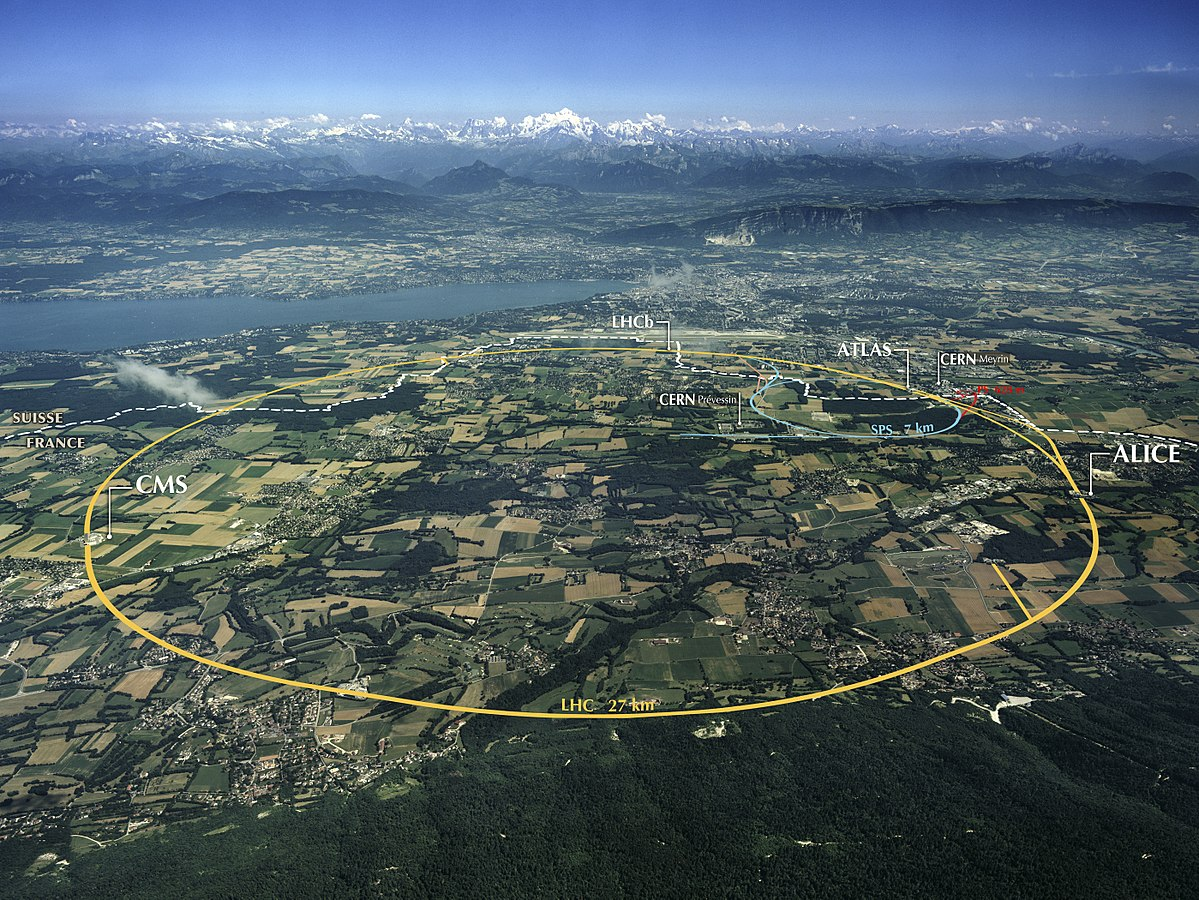
\includegraphics[width=.85\textwidth]{./img/CERN_LHC.jpg}
        \caption{inserire didascalia}
        \label{fig:cern_lhc}
    \end{figure}
\end{frame}

\begin{frame}[fragile]{CMS}
  \begin{figure}
        \centering
        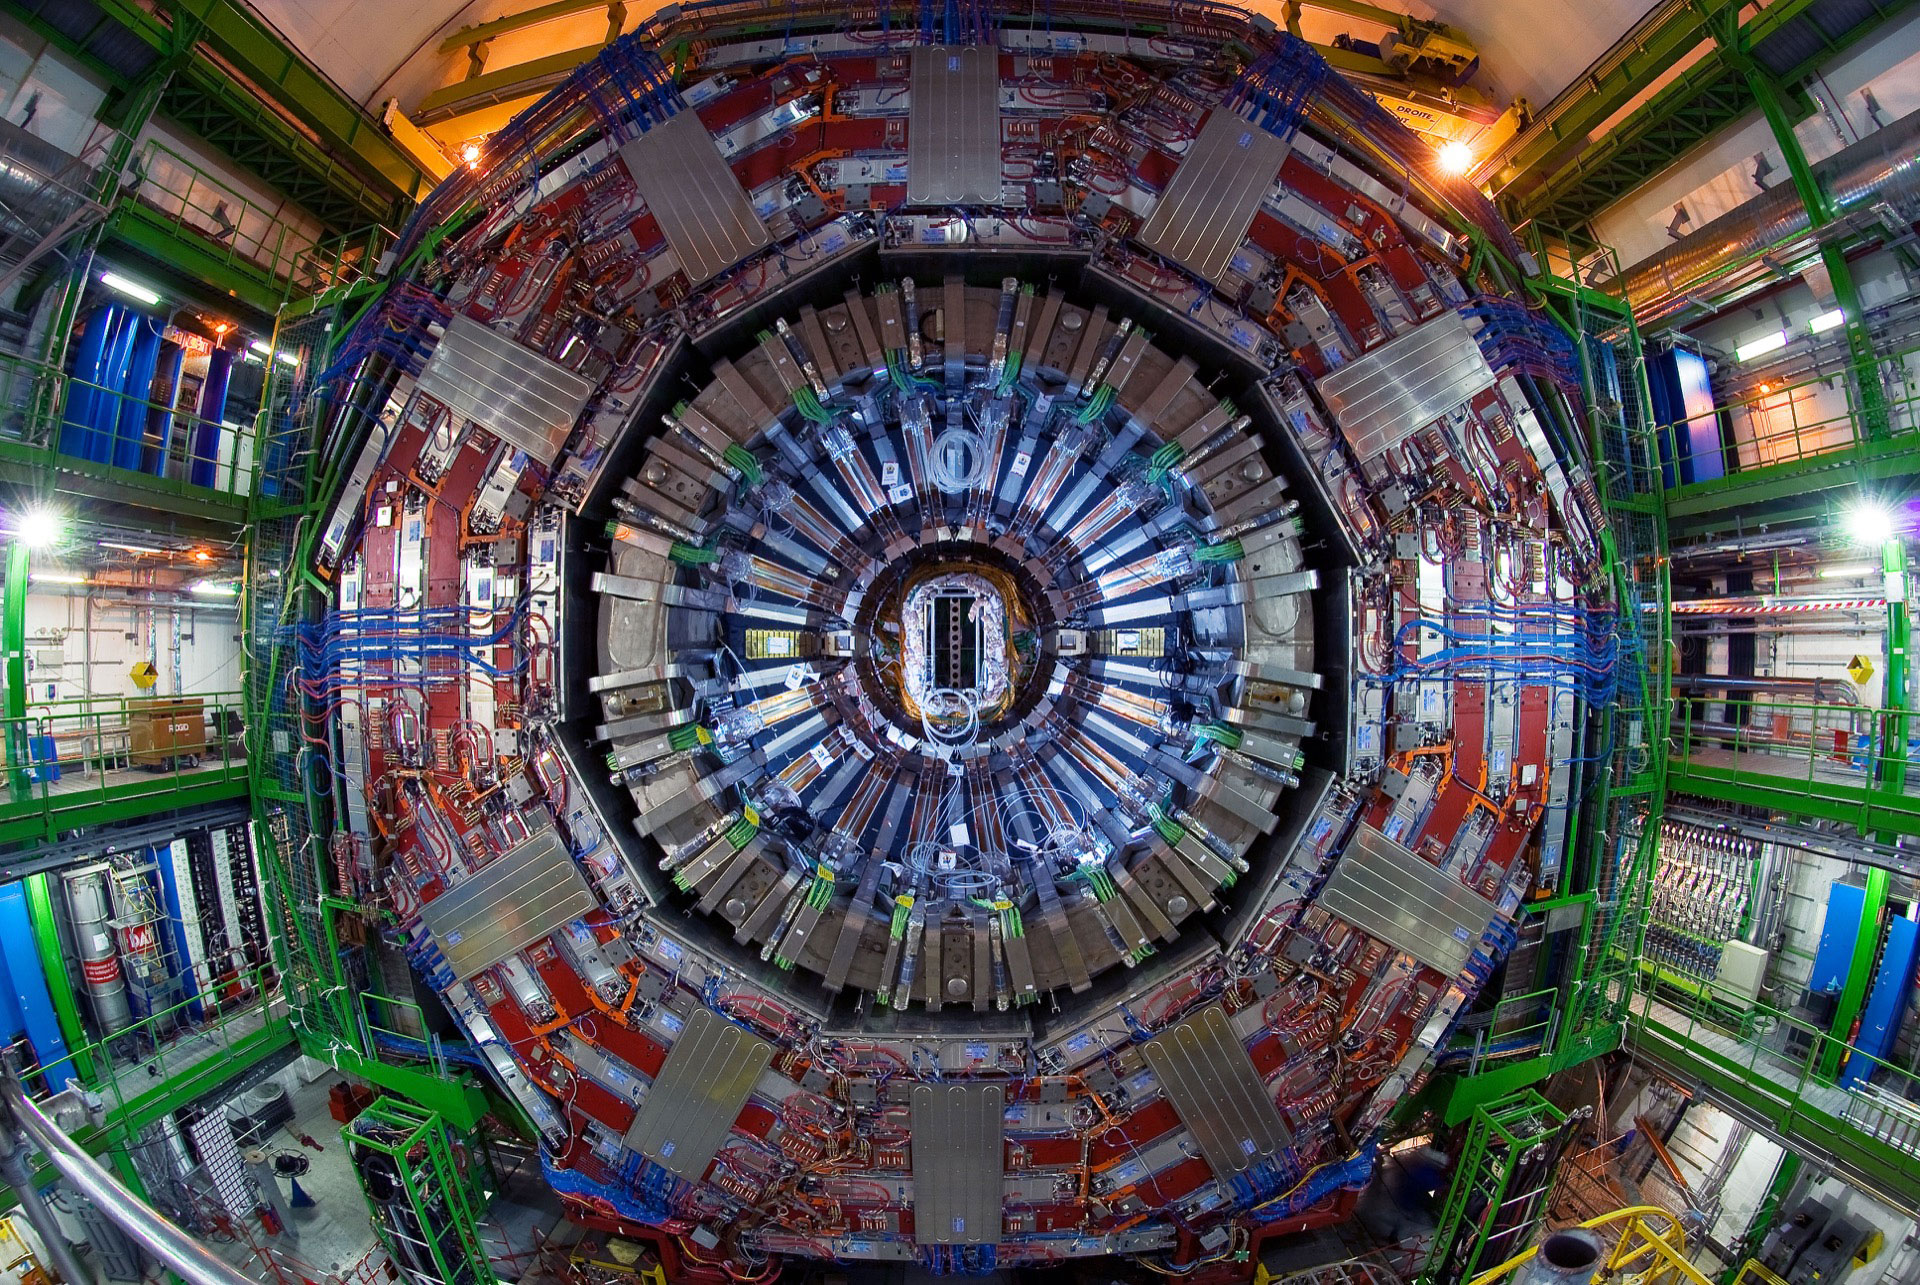
\includegraphics[width=\textwidth]{./img/CMS_front.jpg}
        \caption{CMS experiment section view}
        \label{fig:cms_front}
    \end{figure}
\end{frame}

\begin{frame}[fragile]{CMS}
  \begin{figure}
        \centering
        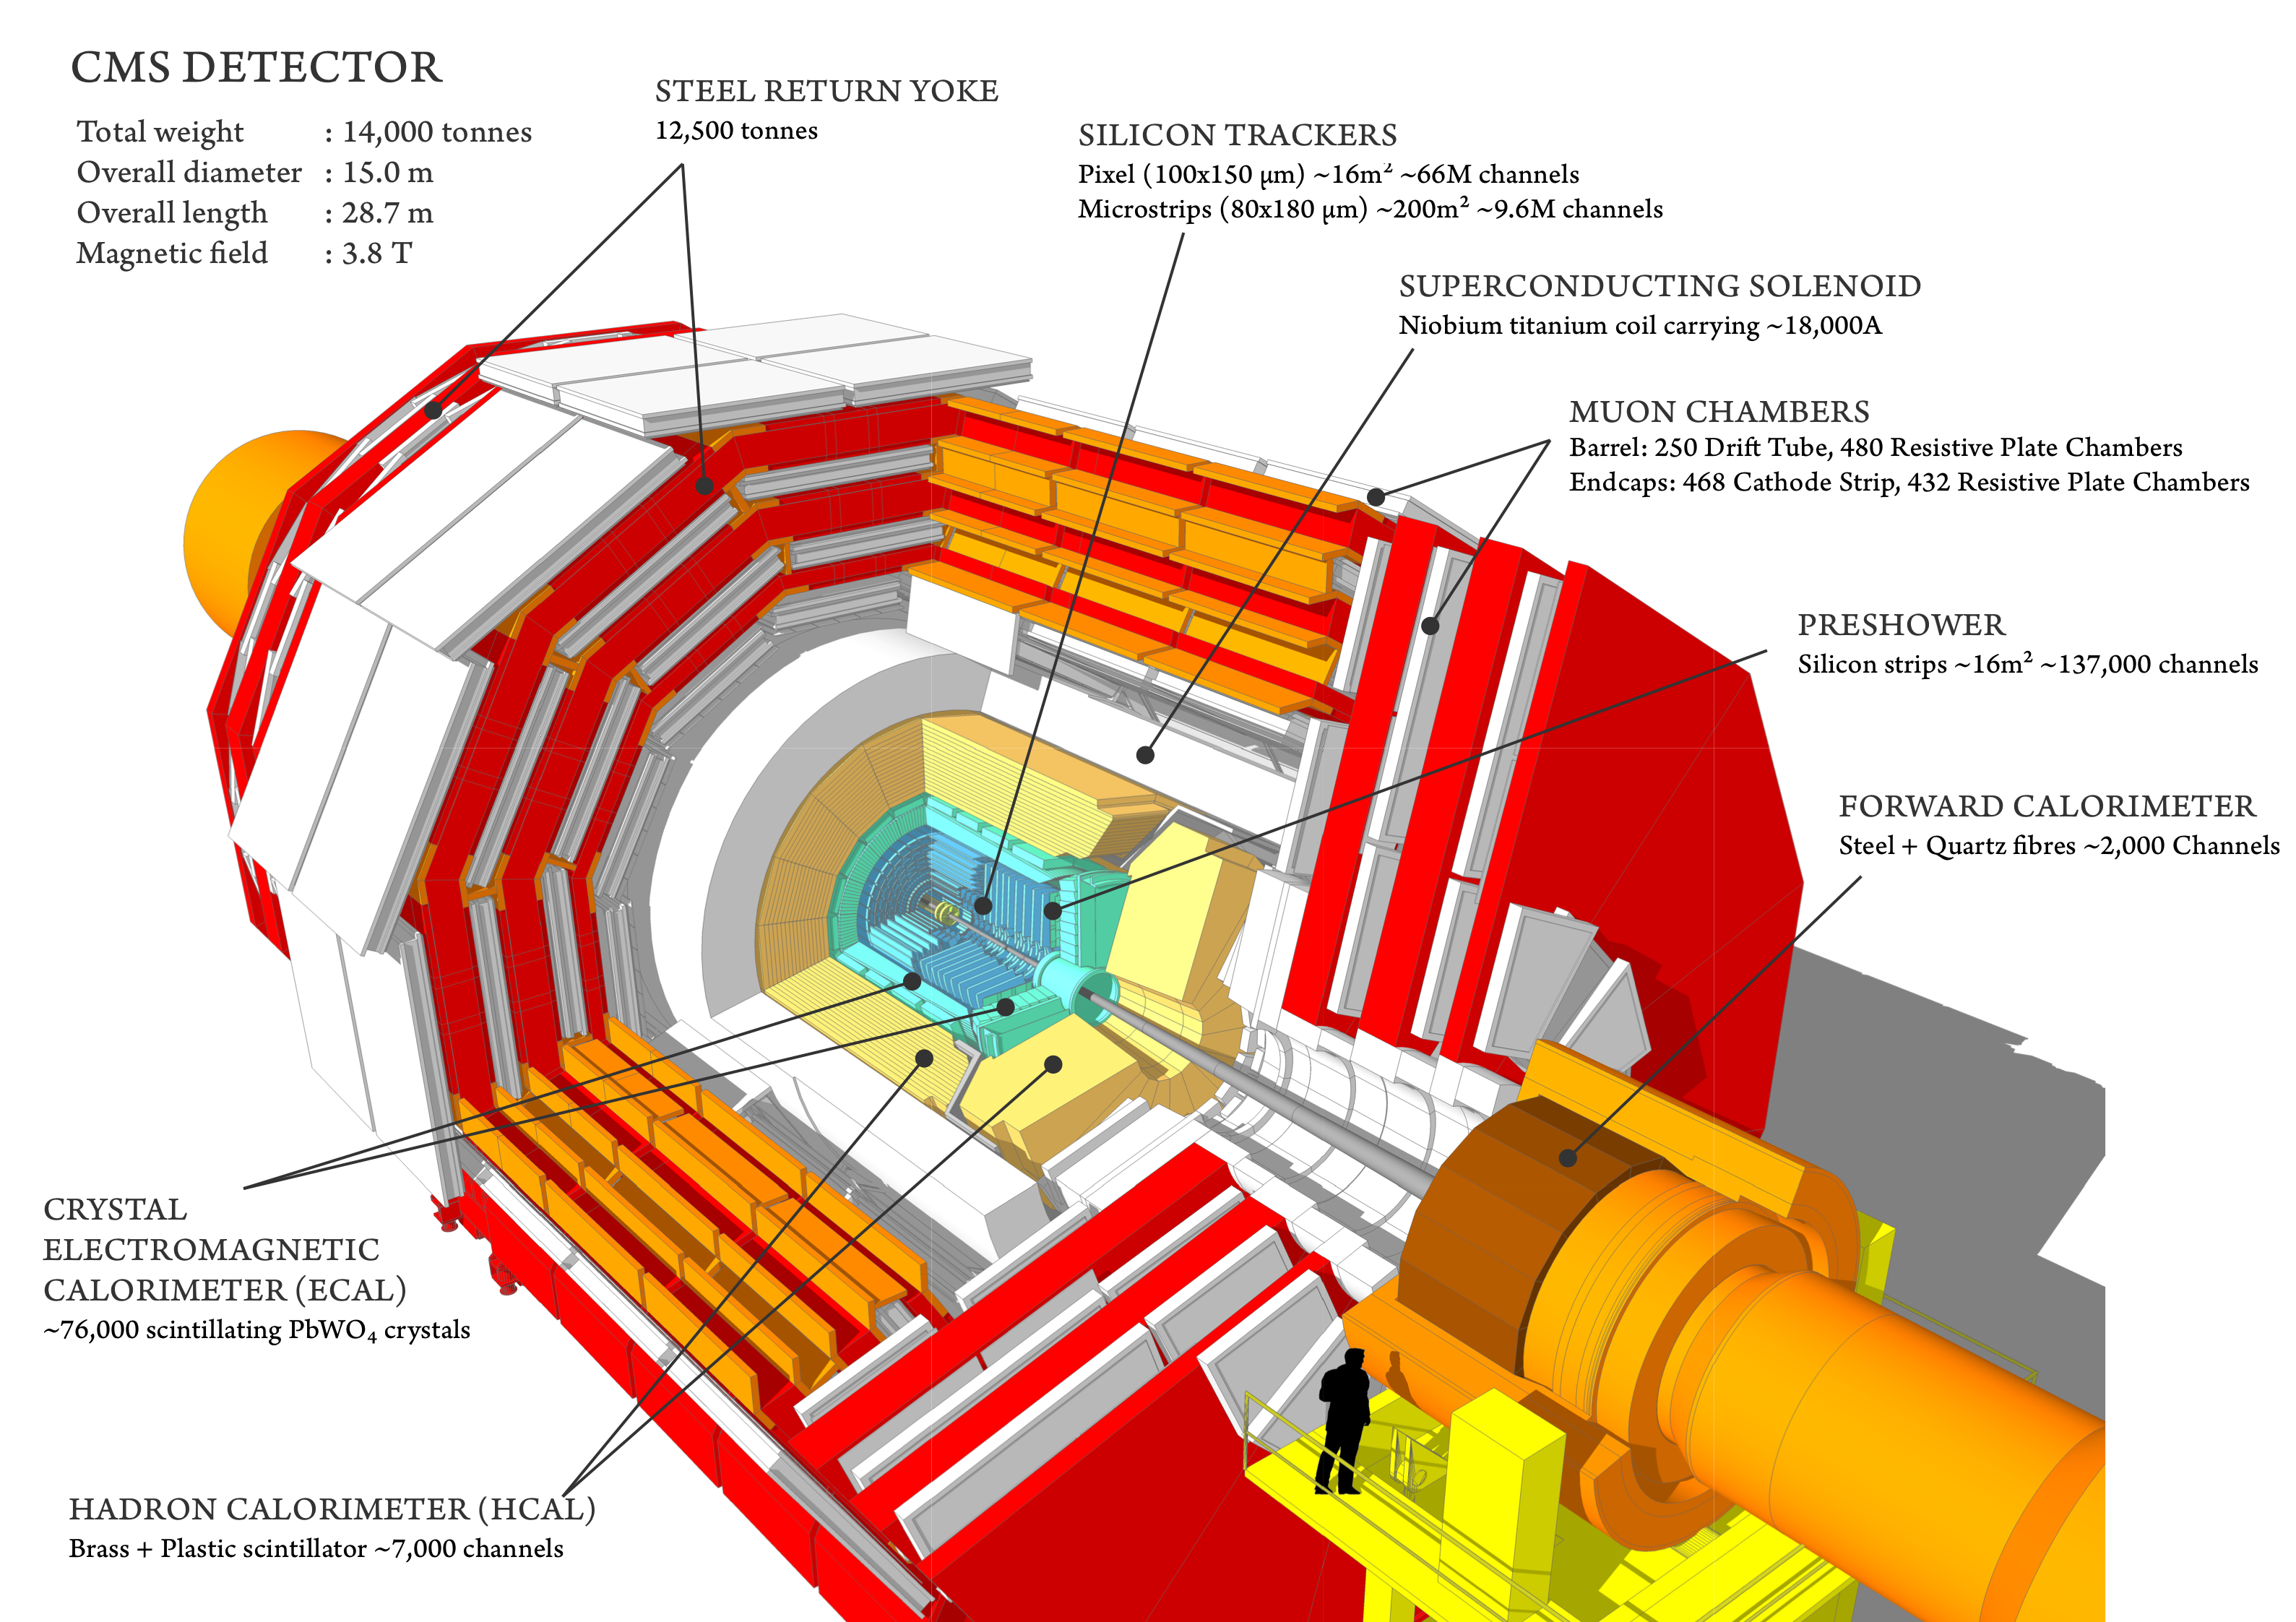
\includegraphics[width=.8\textwidth]{./img/CMS_scheme.png}
        \caption{CMS experiment scheme}
        \label{fig:cms_scheme}
    \end{figure}
\end{frame}


\section{EM Calorimeter}

\begin{frame}[fragile]{EM Calorimeter}



    \textbf{Barrel ECAL}
    \begin{itemize}
        \item  covering $|\eta| \leq 1.479 $ range
        \item $61200$ crystals organized in $5\times5$ modules and $36$ supermodules
        \item $360$-fold in $\phi$ & $(2\times85)$-fold in $\eta$
        \item crystal lenght: $230$\,mm corresponding to $25.8\,X_0$ 
    \end{itemize}
    \textbf{Endcap ECAL} 
    \begin{itemize}
        \item $1.479 \leq |\eta| \leq 3.0 $
        \item Each endcap divided in 2 "Dees", each with 3662 crystals organized in $5\times5$ supercrystals
        \item crystal lenght: $220$\,mm corresponding to $24.7\,X_0$ 
    \end{itemize}
\end{frame}

\begin{frame}{Design}
    \begin{figure}
        \centering
        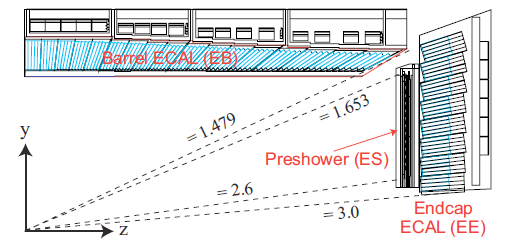
\includegraphics[width=\textwidth]{./img/EMCal_Scheme.png}
        \caption{emcal scheme}
        \label{fig:emcalScheme}
    \end{figure}
\end{frame}

\begin{frame}[fragile]{EM Calorimeter}
  non mi piace molto questa foto, vedi se ne trovi una migliore...
  \begin{figure}
        \centering
        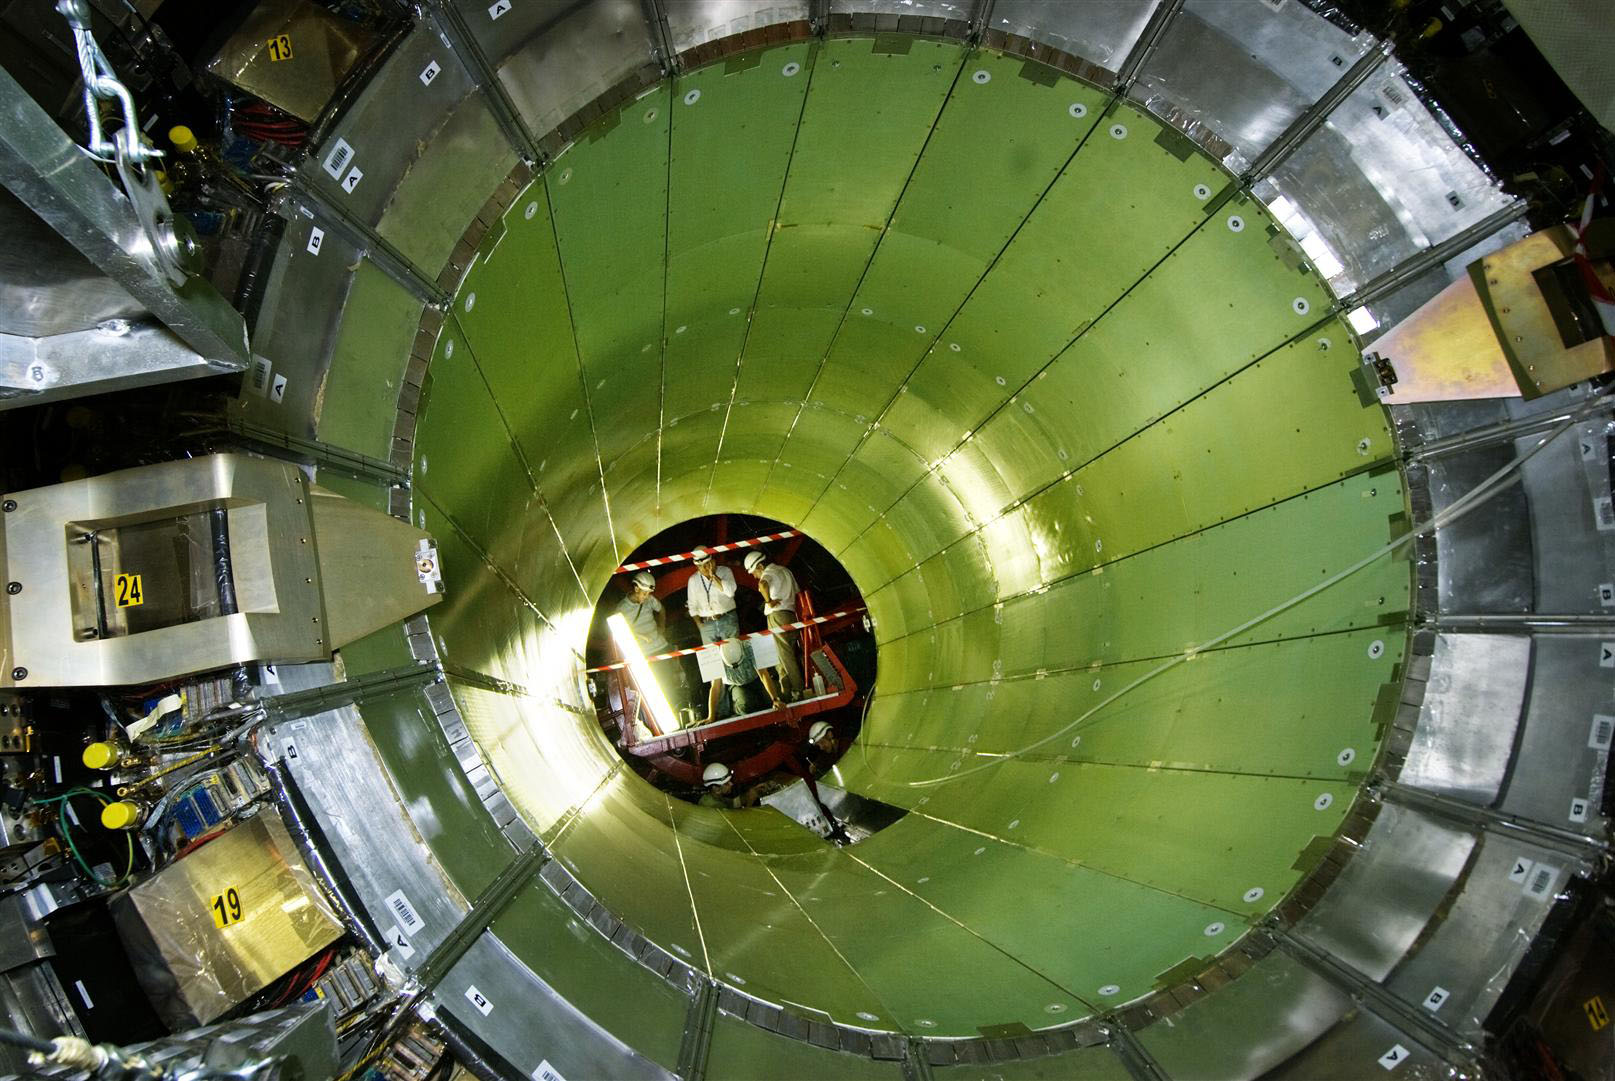
\includegraphics[width=.85\textwidth]{./img/ecal_barrel_photo.jpg}
        \caption{inserire didascalia}
        \label{fig:cms_barrel_photo}
    \end{figure}
\end{frame}

\begin{frame}{Frame Title}
    \begin{figure}
        \centering
        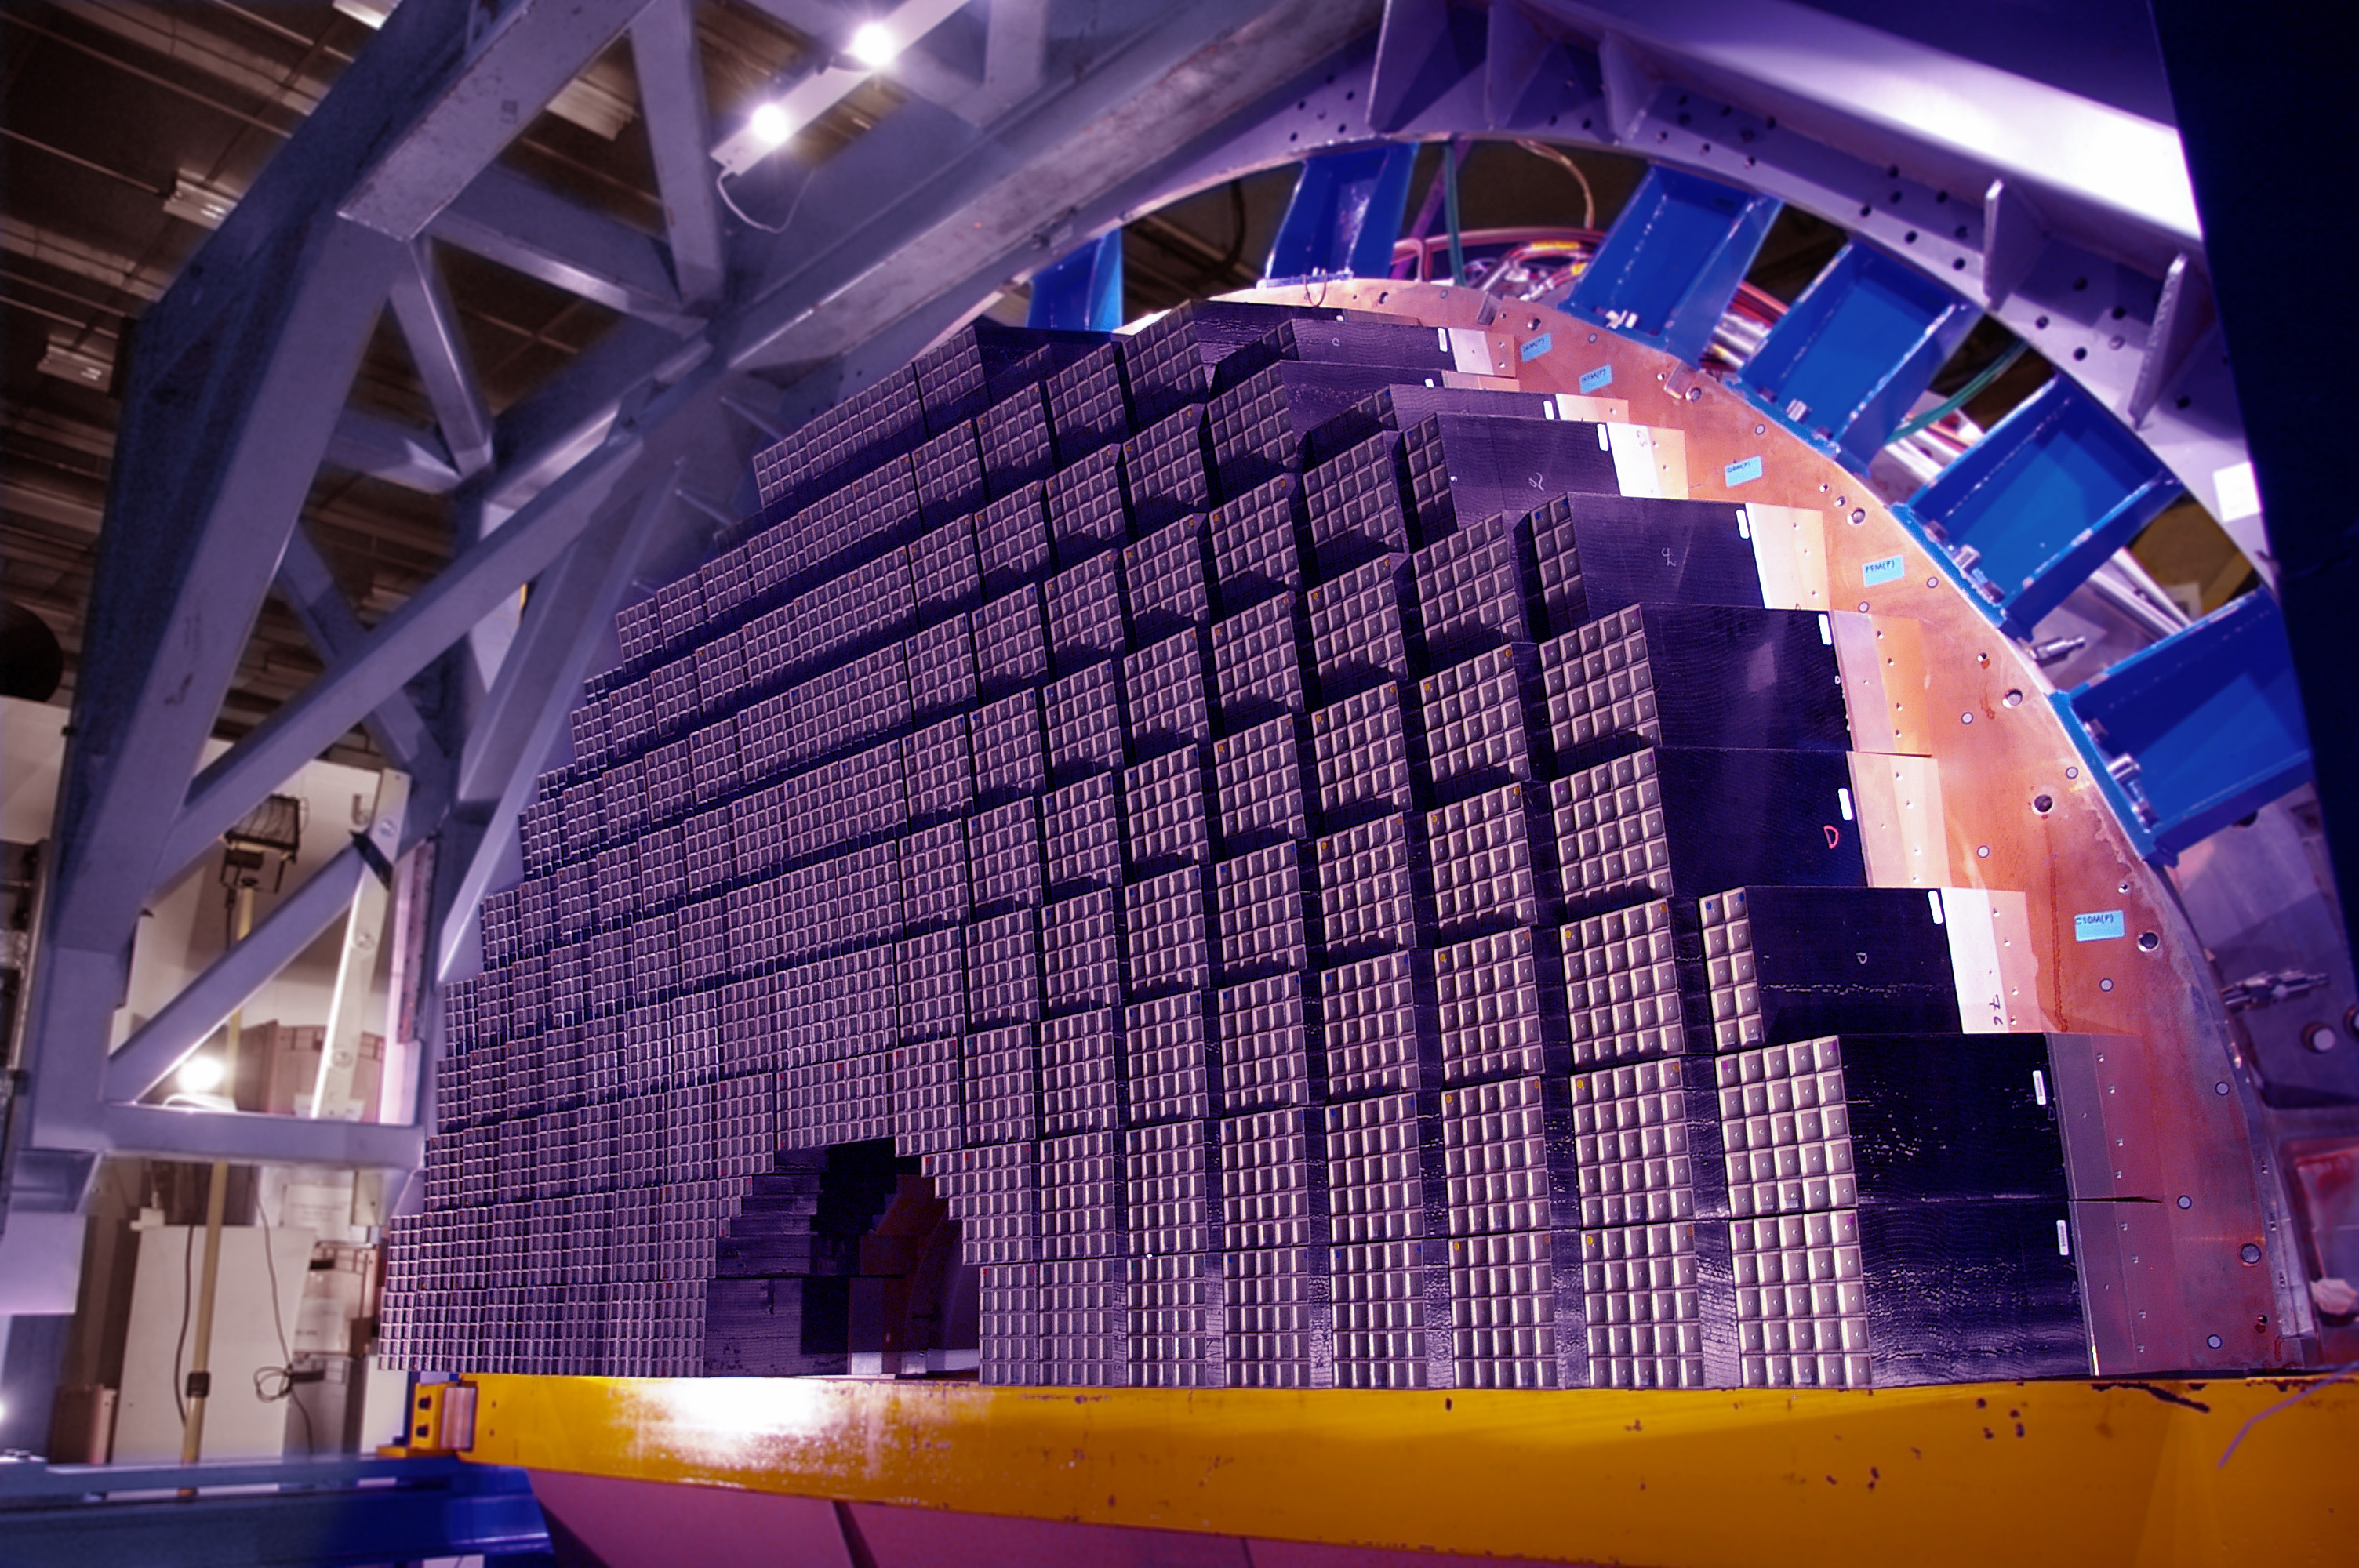
\includegraphics[width=.85\textwidth]{./img/ecal_endcap_photo.jpg}
        \caption{One of the four "Dees" of the endcap EmCal }
        \label{fig:ecal_dees}
    \end{figure}
\end{frame}

\begin{frame}{Design}
    non mi piace molto questa immagine.. ma è un supermodulo del barrel
    \begin{figure}
        \centering
        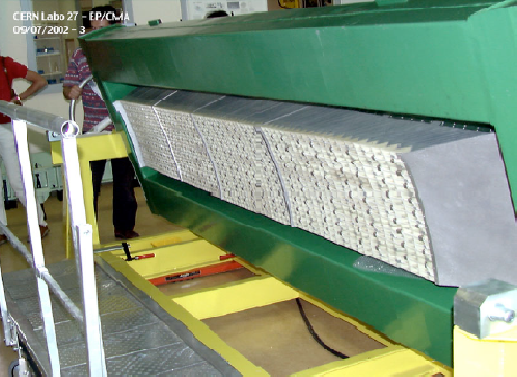
\includegraphics[width=100pt]{./img/emcal_module.png}
        \caption{EmCal module}
        \label{fig:emcalModule}
    \end{figure}
\end{frame}

\begin{frame}{Lead Tungstate ($\text{PbWO}_4$) Crystals}
    \begin{columns}
        \begin{column}[l]{0.40\textwidth}
            \begin{figure}
                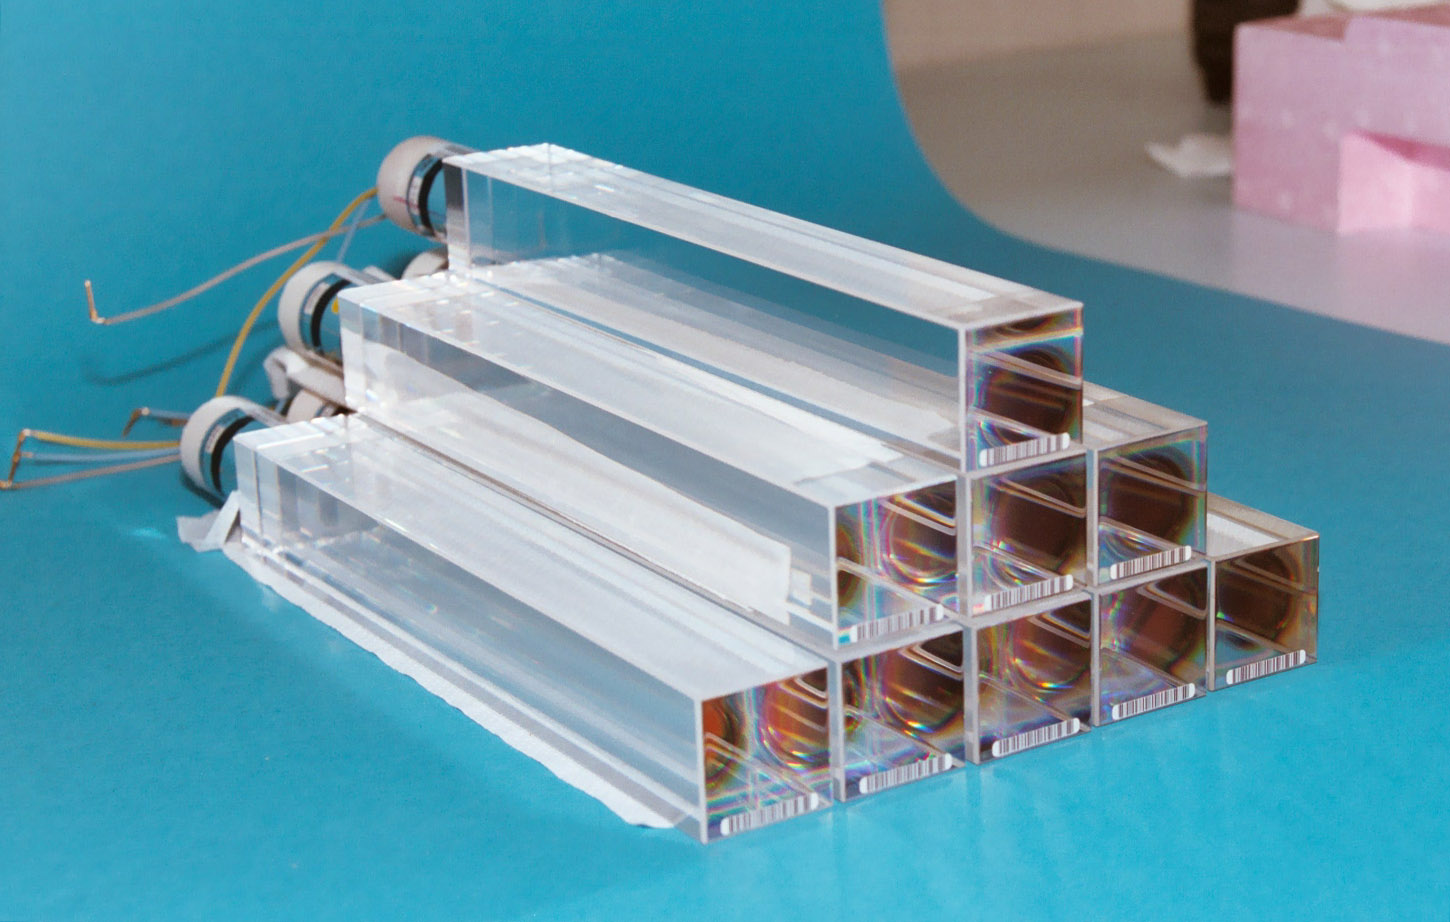
\includegraphics[width=\textwidth]{./img/crystals.jpg}
            \end{figure}    
%            \begin{figure}
%                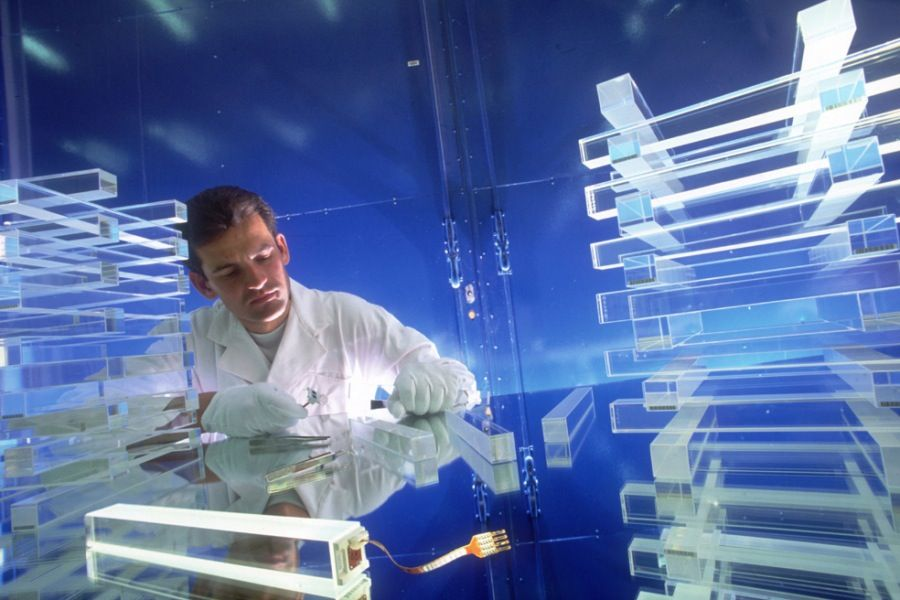
\includegraphics[width=\textwidth]{./img/crystal_production.jpg}
%            \end{figure}    
            \end{column}
        \begin{column}[l]{0.55\textwidth}
        
        \begin{itemize}
                \item $\rho = 8.3\,$g/cm$^3$
                \item $X_0 = 0.89\,$cm
                \item Moliere Radius $ = 2.2$\,cm
                \item Light Output: $4.5$ ph/MeV
                \item Green-Blue light, max @ 420\,nm
                \item Polished for internal reflection
            \end{itemize}
        \end{column}
    \end{columns}
    \bigskip
    \textbf{High radiation levels} throughout the duration of the experiment $\rightarrow$ wavelength dependent loss of light transmission without changes to the scintillation mechanism.
    
    Radiation hardness properties are required: the induced light attenuation length must be always greater than 3$\times$ crystal length. 
    
    Damage is tracked and corrected by a laser light monitoring system.
 
\end{frame}

\begin{frame}{Photodetectors}
    \textbf{Barrel EMCal}
    \begin{itemize}
        \item Reverse structure avalanche photodiodes (APDs)
        \item Glued to the back of the crystals
        \item High quantum efficiency ($\sim 75$\,\%) with mean gain of $50$
    \end{itemize}{}
    
    \textbf{Endcap EMCal}
    \begin{itemize}
        \item Vacuum Phototriodes
        \item Essentially photomultipliers, with a single gain stage
        \item Specially designed to withstand the $4$\,T magnetic field
        \item $22$\,\% quantum efficiency with mean gain of $10.2$ at $0$\,T
    \end{itemize}
\end{frame}

\begin{frame}{Pre-shower Detector}
        fare il preshower, non so quanto approfondirlo, vediamo alla fine se ci sta
\end{frame}

\begin{frame}{Elettronica e Segnale}
    voglio dire qualcosa di elettronica ed elaborazione del segnale? è necessario?
\end{frame}

\begin{frame}{Energy Resolution}
    Showers in EMCal are reconstructed by building \emph{clusters} of crystals. Best performance is obtained using a simple 3x3 (or 5x5) sliding window centered in the crystal having the maximum energy deposition.
    \begin{figure}
        \centering
        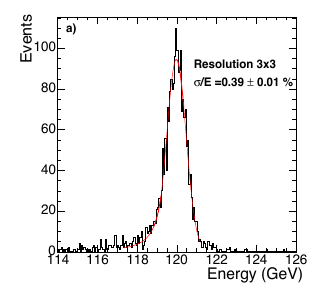
\includegraphics[height=130pt]{./img/resolution_1.png}
        \caption{Energy Distribution reconstructed during the test beam (pointed to the centre of the supermodule).}
        \label{fig:res1}
    \end{figure}{}
\end{frame}

\begin{frame}{Energy Resolution}
    \begin{figure}
        \centering
        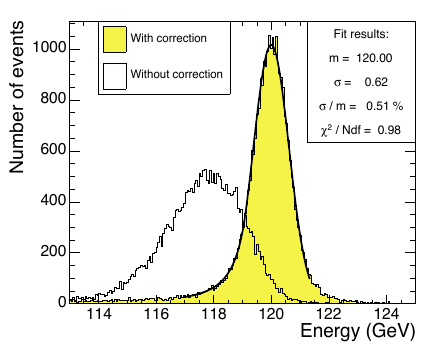
\includegraphics[height=150pt]{./img/resolution_2.png}
        \caption{Energy distribution reconstructed during the test beam (pointed to a \emph{corner} of the supermodule). A single correction function, parametrized from the data, was applied to all regions of the supermodule to take into account variations in shower containment.}
        \label{fig:res2}
    \end{figure}{}
\end{frame}

\begin{frame}{Energy Resolution}
    Energy Resolution can be parametrized as a function of energy
    \begin{equation}
        \biggl(\frac{\sigma}{E}\biggr)^2 = \biggl(\frac{S}{\sqrt{E}}\biggr)^2 + \biggl(\frac{N}{E}\biggr)^2 + C^2 ,
    \end{equation}
  
    \begin{columns}
        \begin{column}[l]{0.45\textwidth}
        \begin{itemize}
            \item S is the \textbf{stochastic} term
            \item N is the \textbf{noise}
            \item C is a \textbf{constant} term
        \end{itemize}
        \end{column}
        \begin{column}[l]{0.45\textwidth}
            \begin{figure}
            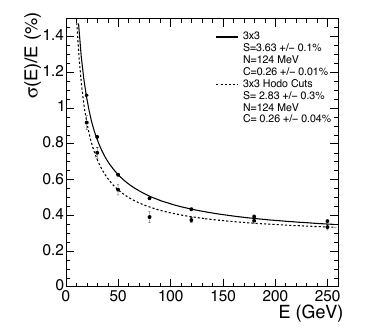
\includegraphics[width=\textwidth]{./img/res_energy.png}
            \end{figure}
        \end{column}
    \end{columns}
    
\end{frame}

\begin{frame}{Calibration}
    It is a \emph{severe technical challenge}.
    Naturally divided in two parts:
    \begin{itemize}
        \item \textbf{Absolute energy scale}
        \item \textbf{Inter-calibration}
    \end{itemize}
    The final energy measurement is given by
    \begin{equation}
        E_{e,\gamma} = G \times \mathcal{F} \times \sum_i c_i \times A_i
    \end{equation}
    where
    \begin{itemize}
        \item $G$ is a \emph{global absolute scale}
        \item $\mathcal{F}$ is a \emph{correction function} depending on particle type, position, momentum...
        \item $c_i$ are the \emph{inter-calibration coefficients}
        \item $A_i$ are the \emph{signal amplitudes} summed over the cluster of crystals 
    \end{itemize}{}
    
\end{frame}

\begin{frame}{Inter-calibration}
    Calibration between different crystals of the calorimeter relatively to the absolute energy scale.
    
    Measured with various methods:
    \begin{itemize}
        \item \textbf{Phi independence} Taking advantage of the $\phi$ symmetry of deposited energy to inter-calibrate crystal rings at constant $\eta$.
        \item \textbf{Single electrons} Exploiting single electrons $p$ measurements from the \emph{tracker} to inter-calibrate different crystals in a single module.
        \item \textbf{$\text{Z} \rightarrow \text{ee}$} Reconstruction of the $ee$ invariant mass and calibration exploiting the $Z$ mass constraint, studying the distribution of 
        \begin{equation}
            \epsilon^i = \frac{1}{2} \biggl[\biggl(\frac{M^i_\text{inv}}{M_Z}\biggr)^2 - 1\biggr]
        \end{equation}{}
    \end{itemize}{}
    
\end{frame}

\begin{frame}{Inter-calibration}
    \begin{figure}
        \centering
        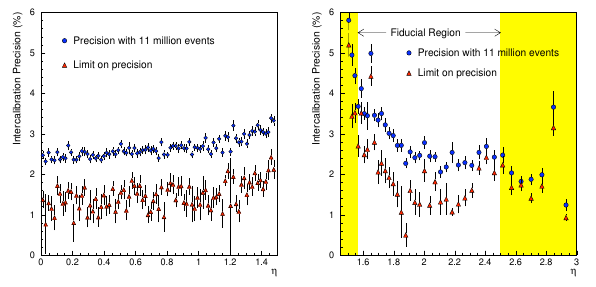
\includegraphics[height=150pt]{./img/intercalib_phi.png}
        \caption{Intercalibration precision as function on $\eta$, for barrel and endcap.}
        \label{fig:intercalib_phi}
    \end{figure}
    
    immagini per Se e Zee
\end{frame}{}

\section{HL-LHC Upgrade}


\begin{frame}{Conclusion}
    \begin{itemize}
        \item one
        \item two
    \end{itemize}
\end{frame}
 
\end{document}
